% !TEX TS-program = pdflatexmk
\documentclass[12pt]{amsart}
\usepackage[letterpaper, portrait, left = 1in, right = 1in, top = 1.2in, bottom=1.5in]{geometry} 
%\usepackage{setspace} \doublespacing
%\usepackage[letterpaper, portrait, margin=1.3in]{geometry}
\usepackage[table,xcdraw]{xcolor}
\usepackage{amssymb}
\usepackage{amsfonts}
\usepackage{longtable}
\usepackage{amsmath,amsthm}
\usepackage{enumitem}
\usepackage[utf8]{inputenc}
\usepackage{mathtools}
\usepackage{graphicx}
\usepackage{parskip}
\usepackage{multicol}
\usepackage{listings}
\usepackage[skip=0.25pt]{caption}
\usepackage[mathscr]{euscript}
\usepackage{quiver}
\setlength{\parindent}{0pt}
\usepackage{thm-restate}
\definecolor{vividburgundy}{rgb}{0.62, 0.11, 0.21}
\usepackage[driverfallback=hypertex,pagebackref=false,colorlinks,citecolor=vividburgundy]{hyperref}
\usepackage[capitalize]{cleveref}
%\usepackage[cmintegrals,cmbraces]{newtxmath}
%\usepackage{ebgaramond-maths}

%\usepackage{fourier}
%----------FONT OPTIONS----------
% sans-serif
%\usepackage[sfdefault]{FiraSans}
 %\usepackage[sfdefault]{roboto}
% \usepackage[sfdefault]{noto-sans}
%\usepackage[default]{sourcesanspro}

% serif
%\usepackage{CormorantGaramond}

%\usepackage{charter}
\usepackage[T1]{fontenc}
\usepackage{cleveref}
\definecolor{dg}{RGB}{10, 100, 10}
\setlength{\parindent}{0in}
\renewcommand{\qed}{$\hfill\blacksquare$}
% \newtheoremstyle{style}{2pt}{1pt}{\normalfont}{}{\bfseries}{\\}{0cm}{}
% \theoremstyle{style}
\newtheorem{lemma}{Lemma}[section]
% \newtheorem{lemma}{Lemma}
\newtheorem{thm}[lemma]{Theorem}
\newtheorem{prop}[lemma]{Proposition}
\newtheorem{cor}[lemma]{Corollary}
\newtheorem{conj}[lemma]{Conjecture}
\newtheorem{cl}[lemma]{Claim}
\newtheorem{rmk}{Remark}
\newtheorem{defn}[lemma]{Definition}
\newtheorem{qs}{Question}
\newtheoremstyle{styleS}{}{}{\color{dg}}{}{\color{dg}\bfseries}{. }{0cm}{}
\theoremstyle{styleS}
\newtheorem*{sol}{Solution}
\newtheoremstyle{style1}{}{}{\normalfont}{}{\bfseries}{. }{0cm}{}
\theoremstyle{style1}
\newtheorem{prob}{Problem}[section]
\newtheorem*{prb}{Problem}
\newtheoremstyle{style2}{1pt}{4pt}{\normalfont}{}{\itshape}{. }{0cm}{}
\theoremstyle{style2}
\newtheorem{ex}[lemma]{Example}
\newtheorem*{pf}{Proof}

\newcommand{\norm}[2]{
\left\lVert #1 \right\rVert_{#2}
}
\usepackage{mathrsfs}
%\usepackage[table,xcdraw]{xcolor}
\usepackage{booktabs}
\usepackage{tikz}
\usetikzlibrary{matrix}
\renewcommand{\l}{\ell}


\newcommand{\fA}{{\mathfrak{A}}}   \newcommand{\fB}{{\mathfrak{B}}}
\newcommand{\fC}{{\mathfrak{C}}}   \newcommand{\fD}{{\mathfrak{D}}}
\newcommand{\fE}{{\mathfrak{E}}}   \newcommand{\fF}{{\mathfrak{F}}}
\newcommand{\fG}{{\mathfrak{G}}}   \newcommand{\fH}{{\mathfrak{H}}}
\newcommand{\fI}{{\mathfrak{I}}}   \newcommand{\fJ}{{\mathfrak{J}}}
\newcommand{\fK}{{\mathfrak{K}}}   \newcommand{\fL}{{\mathfrak{L}}}
\newcommand{\fM}{{\mathfrak{M}}}   \newcommand{\fN}{{\mathfrak{N}}}
\newcommand{\fO}{{\mathfrak{O}}}   \newcommand{\fP}{{\mathfrak{P}}}
\newcommand{\fQ}{{\mathfrak{Q}}}   \newcommand{\fR}{{\mathfrak{R}}}
\newcommand{\fS}{{\mathfrak{S}}}   \newcommand{\fT}{{\mathfrak{T}}}
\newcommand{\fU}{{\mathfrak{U}}}   \newcommand{\fV}{{\mathfrak{V}}}
\newcommand{\fW}{{\mathfrak{W}}}   \newcommand{\fX}{{\mathfrak{X}}}
\newcommand{\fY}{{\mathfrak{Y}}}   \newcommand{\fZ}{{\mathfrak{Z}}}

\newcommand{\cA}{{\mathcal{A}}}   \newcommand{\cB}{{\mathcal{B}}}
\newcommand{\cC}{{\mathcal{C}}}   \newcommand{\cD}{{\mathcal{D}}}
\newcommand{\cE}{{\mathcal{E}}}   \newcommand{\cF}{{\mathcal{F}}}
\newcommand{\cG}{{\mathcal{G}}}   \newcommand{\cH}{{\mathcal{H}}}
\newcommand{\cI}{{\mathcal{I}}}   \newcommand{\cJ}{{\mathcal{J}}}
\newcommand{\cK}{{\mathcal{K}}}   \newcommand{\cL}{{\mathcal{L}}}
\newcommand{\cM}{{\mathcal{M}}}   \newcommand{\cN}{{\mathcal{N}}}
\newcommand{\cO}{{\mathcal{O}}}   \newcommand{\cP}{{\mathcal{P}}}
\newcommand{\cQ}{{\mathcal{Q}}}   \newcommand{\cR}{{\mathcal{R}}}
\newcommand{\cS}{{\mathcal{S}}}   \newcommand{\cT}{{\mathcal{T}}}
\newcommand{\cU}{{\mathcal{U}}}   \newcommand{\cV}{{\mathcal{V}}}
\newcommand{\cW}{{\mathcal{W}}}   \newcommand{\cX}{{\mathcal{X}}}
\newcommand{\cY}{{\mathcal{Y}}}   \newcommand{\cZ}{{\mathcal{Z}}}

\newcommand{\sA}{{\mathscr{A}}}   \newcommand{\sB}{{\mathscr{B}}}
\newcommand{\sC}{{\mathscr{C}}}   \newcommand{\sD}{{\mathscr{D}}}
\newcommand{\sE}{{\mathscr{E}}}   \newcommand{\sF}{{\mathscr{F}}}
\newcommand{\sG}{{\mathscr{G}}}   \newcommand{\sH}{{\mathscr{H}}}
\newcommand{\sI}{{\mathscr{I}}}   \newcommand{\sJ}{{\mathscr{J}}}
\newcommand{\sK}{{\mathscr{K}}}   \newcommand{\sL}{{\mathscr{L}}}
\newcommand{\sM}{{\mathscr{M}}}   \newcommand{\sN}{{\mathscr{N}}}
\newcommand{\sO}{{\mathscr{O}}}   \newcommand{\sP}{{\mathscr{P}}}
\newcommand{\sQ}{{\mathscr{Q}}}   \newcommand{\sR}{{\mathscr{R}}}
\newcommand{\sS}{{\mathscr{S}}}   \newcommand{\sT}{{\mathscr{T}}}
\newcommand{\sU}{{\mathscr{U}}}   \newcommand{\sV}{{\mathscr{V}}}
\newcommand{\sW}{{\mathscr{W}}}   \newcommand{\sX}{{\mathscr{X}}}
\newcommand{\sY}{{\mathscr{Y}}}   \newcommand{\sZ}{{\mathscr{Z}}}

\newcommand{\ta}{{\tilde{a}}}   \newcommand{\tb}{{\tilde{b}}}
\newcommand{\tc}{{\tilde{c}}}   \newcommand{\td}{{\tilde{d}}}
\newcommand{\te}{{\tilde{e}}}   \newcommand{\tf}{{\tilde{f}}}
\newcommand{\tg}{{\tilde{g}}}   
\newcommand{\ti}{{\tilde{i}}}   \newcommand{\tj}{{\tilde{j}}}
\newcommand{\tk}{{\tilde{k}}}   \newcommand{\tl}{{\tilde{l}}}
\newcommand{\tm}{{\tilde{m}}}   \newcommand{\tn}{{\tilde{n}}}
		         	\newcommand{\tp}{{\tilde{p}}}
\newcommand{\tq}{{\tilde{q}}}   \newcommand{\tr}{{\tilde{r}}}
\newcommand{\ts}{{\tilde{s}}}   
\newcommand{\tu}{{\tilde{u}}}   \newcommand{\tv}{{\tilde{v}}}
\newcommand{\tw}{{\tilde{w}}}   \newcommand{\tx}{{\tilde{x}}}
\newcommand{\ty}{{\tilde{y}}}   \newcommand{\tz}{{\tilde{z}}}

\newcommand{\red}{{\color{red}red}}
\newcommand{\blue}{{\color{blue}blue}}

\newcommand{\into}{\hookrightarrow}
\newcommand{\onto}{\twoheadrightarrow}
\newcommand\N{\ensuremath{\mathbb{N}}}

%\newcommand\L{\ensuremath{\mathbb{L}}}
\newcommand{\bP}{\mathbb{P}}
\newcommand\M{\ensuremath{\mathbb{M}}}
\newcommand\R{\ensuremath{\mathbb{R}}}
\newcommand\Z{\ensuremath{\mathbb{Z}}}
\renewcommand\O{\ensuremath{\emptyset}}
\newcommand\Q{\ensuremath{\mathbb{Q}}}
\newcommand\C{\ensuremath{\mathbb{C}}}
\newcommand{\K}{\ensuremath{\mathbb{K}}}
\newcommand\F{\ensuremath{\mathbb{F}}}
\newcommand{\aff}{\ensuremath{\mathbb{A}}}
\newcommand{\proj}{\ensuremath{\mathbb{P}}}
\newcommand{\dd}{\mathrm{d}}
\newcommand{\m}{\ensuremath{\mathfrak{m}}}
\newcommand{\p}{\ensuremath{\mathfrak{p}}}
\newcommand{\n}{\ensuremath{\mathfrak{n}}}
\renewcommand{\phi}{\varphi}
\renewcommand{\qedsymbol}{\ensuremath{\blacksquare}}
%\newcommand{\st}{\;|\;}
\newcommand{\st}{%
  \nonscript\;
  \ifnum\currentgrouptype=16
    \;\middle|\;
  \else
    \;|\;
  \fi
  \nonscript\;}
\newcommand{\ltr}{\par \noindent \framebox[1\width]{ $\implies$ } \hspace{.2cm}}
\newcommand{\rtl}{\par \noindent \framebox[1\width]{ $\impliedby$ } \hspace{.2cm} }
\newcommand{\abs}[1]{\left| #1 \right|}
\newcommand{\inner}[2]{\left\langle #1, #2 \right\rangle}
\newcommand{\E}[1]{\mathbb E\left[ #1 \right]}
\newcommand{\e}[1]{\exp\left( #1 \right)}
\renewcommand{\P}[1]{\mathbb P\left[ #1 \right]}
\newcommand{\Var}[1]{\text{Var}\left[ #1 \right]}
\newcommand*\circled[1]{\tikz[baseline=(char.base)]{
            \node[shape=circle,draw,inner sep=2pt] (char) {#1};}}
\newcommand{\ds}{\displaystyle}

\DeclareMathOperator{\sym}{Sym}
\DeclareMathOperator{\mds}{MDS}
\DeclareMathOperator{\Tor}{Tor}
\DeclareMathOperator{\Ext}{Ext}
\DeclareMathOperator{\adj}{adj}
\DeclareMathOperator{\Tr}{Tr}
\DeclareMathOperator{\GL}{GL}
%\DeclareMathOperator{\Tr}{Tr}
\DeclareMathOperator{\orbit}{Or}
\DeclareMathOperator{\stab}{Stab}
\DeclareMathOperator{\fix}{Fix}
\DeclareMathOperator{\re}{Re}
\DeclareMathOperator{\im}{Im}
\DeclareMathOperator{\ord}{Ord}
\DeclareMathOperator{\mspec}{mSpec}
\DeclareMathOperator{\spec}{Spec}
\DeclareMathOperator{\frob}{Frob}
\DeclareMathOperator{\id}{Id}
\DeclareMathOperator{\colim}{colim}
\DeclareMathOperator{\loc}{loc}
\DeclareMathOperator{\res}{Res}
\DeclareMathOperator{\rad}{rad}
\DeclareMathOperator{\Res}{Res}
\DeclareMathOperator{\diam}{diam}
\DeclareMathOperator{\arcsec}{arcsec}
\DeclareMathOperator{\arccot}{arccot}
\DeclareMathOperator{\len}{len}
\DeclareMathOperator{\area}{area}
\DeclareMathOperator{\vol}{vol}
\DeclareMathOperator{\ev}{ev}
\DeclareMathOperator{\sgn}{sgn}
\DeclareMathOperator{\supp}{supp}
\DeclareMathOperator{\diff}{d}
\DeclareMathOperator{\Dom}{Dom}
\DeclareMathOperator{\rk}{rank}
\renewcommand{\d}{\diff}
\let\oldend\endlinechar
\renewcommand{\endlinechar}{\oldend}
\newcommand{\open}{\underset{\text{open}}{\subset}}
\newcommand{\divides}{\mathbin{|}}
\newcommand{\set}[1]{\ensuremath{\left\{#1\right\}}}
\newcommand{\sett}{\coloneqq}
\newcommand*\isomap{%
  \xrightarrow{\raisebox{-0.9ex}[0ex][0ex]{$\sim$}}%
}
\renewcommand{\epsilon}{\varepsilon}
\newcommand{\fa}{~\forall~}
%\usepackage[nobottomtitles*]{titlesec}
\usepackage{titletoc}
%\titleformat{\section}[runin]
%{\normalfont\Large\bfseries}
%{}{0pt}{}%
%[\ifthenelse{\equal{\thesection}{0}}{\\\vspace*{0pt}}{\space\thesection}]
\newcommand{\sint}{\sin\theta}
\newcommand{\cost}{\cos\theta}
\newcommand{\tant}{\tan\theta}
\newcommand{\lb}{\left[}
\newcommand{\rb}{\right]}
\newcommand{\lp}{\left(}
\newcommand{\rp}{\right)}
\newcommand{\br}[1]{\lb#1\rb}
\newcommand{\pa}[1]{\lp#1\rp}
\usepackage{pdfpages}
\usepackage{fancyhdr}
	\pagestyle{fancyplain}
	\fancyhf{}
	\fancyhead[C]{\thepage}

\usepackage{wrapfig}
\setlength{\columnsep}{0.7cm}
%\fontfamily{qcr}\selectfont 
%\usepackage[backend=bibtex]{biblatex}

%\usepackage[
%backend=biber,
%style=alphabetic,giveninits,
%citestyle=ieee-alphabetic,
%natbib=true,
%uniquelist=false,
%maxnames=10,
%sorting=ynt
%]{biblatex}

\usepackage[
backend=biber,
style=alphabetic,
]{biblatex}
\addbibresource{ref.bib}
%\title{\vspace{-1cm}}
\title{\textbf{Physics of Learning Theory}\\ Lecture $1$ \\
Probability and Learning Theory review}
\usepackage{quiver}
\usepackage[nobottomtitles*]{titlesec}
\usepackage{titletoc}
%\titleformat{\section}[runin]
%  {\normalfont\Large\bfseries}
%  {}{0pt}{}%
%  [\ifthenelse{\equal{\thesection}{0}}{\\\vspace*{0pt}}{\space\thesection}]
%\author{{\Large NILAVA METYA} \\ 
%\href{mailto:nilava.metya@rutgers.edu}{nilava.metya@rutgers.edu}\\
%\href{mailto:nm8188@princeton.edu}{nm8188@princeton.edu}}
\author{Nilava Metya}
\date{\vspace{-0.7in}January $29$, $2025$}
%\newcommand{\pb}{\section{Problem}~\par}
%\newcommand{\soln}{\subsection*{Solution}}
\usepackage{pdfpages}
\usepackage{fancyhdr}
	\pagestyle{fancyplain}
	\fancyhf{}
	\fancyhead[R]{\thepage}
\newcommand{\fa}{~\forall~}
\usepackage{algpseudocode}
\renewcommand{\algorithmicrequire}{\textbf{Input:}}
\renewcommand{\algorithmicensure}{\textbf{Output:}}
\algdef{SE}{Begin}{End}{\textbf{begin}}{\textbf{end}}
\begin{document}

\maketitle

\section{Introduction}
We will recall some probability theory and look at useful \textit{deviation} or \textit{concentration} bounds which are frequently used in analyzing algorithms (in learning theory). Recall that a (real-valued) random variable on a probability space $(\Omega,S,\mathbb P)$ is nothing but a `measurable function' $X:\Omega\to \R$. Here $\Omega$ is the universal or sample space where we think of events in, $S$ is a collection of events in $\Omega$ and $\mathbb P:S\to[0,1]$ assigns probability to each event in $S$. The space of events $S$ is constrained to satisfy some obvious rules like $\Omega$ is an event, if $A$ is an event then so is $\Omega\smallsetminus A$ and that a countable union of events is an event which makes it sensible to work with the concept of assigning probabilities to each event. We will often say that $\P{A}$ is the probability that event $A$ occurs. If $A=\set{a}$ is a singleton, we always write $\P{a}$ instead of $\P{\set{a}}$. The probability function $\mathbb P$ is also constrained to a couple of rules, namely, that the probability of the union of a mutually disjoint collection of events, which is an event, is the same as the sum of the probabilities of each of those events and that the probability that $\Omega$ occurs is $1$. Roughly a random variable is to be thought of as a way of assigning points of the sample space to real numbers which are \textit{really real} and are more tangible to work with, while respecting the rules of $S$. Such a random variable induces a map $X^{-1}:2^{\R}\to S$ by $X^{-1}(A) \sett \set{x\in \Omega\st X(x) \in S}$ for any $A\subseteq \R$, and hence induces a probability on $\R$ given by $\mathbb P_{\R}[A] = \P{X^{-1}(A)}$ where $A$ is any `measurable' subset of $\R$. The random variable being a `measurable function' precisely means that $X^{-1}(A)$ always lies in $S$.
\[\begin{tikzcd}
	S & {2^\R} \\
	{[0,1]}
	\arrow["{\mathbb P}"', from=1-1, to=2-1]
	\arrow["{X^{-1}}"', from=1-2, to=1-1]
	\arrow["{\mathbb P_\R}", dashed, from=1-2, to=2-1]
\end{tikzcd}\]

\subsection{Mean}
The average or mean of a random variable $X$, often denoted as $\E X$, $\mu(X)$, or simply $\mu$ when the context is clear,  is $\E X = \int_{\Omega}  X \d\mathbb P $. For the discrete case, which we will mostly be interested in, this boils down to $\E X = \sum\limits_{i\in \Omega}X(i)\P{i}$. Note that if $X$ is an indicator random variable for event $A$, that is, $X=1$ if $A$ occurs and $0$ otherwise, then $\E X = \P A$.

\begin{ex}
Consider tossing a fair coin. Here $\Omega=\set{\text H, \text T}$. The probability function is $\P{\varnothing}=0, \P{\text H}=\P{\text T}=0.5, \P{\set{\text H,\text T}}=1$. A natural random variable to consider is $X(i) = \pmb 1_{\text H} \sett \begin{cases}1&\text{ if } i=\text H\\0&\text{ if } i=\text T\end{cases}$. The corresponding probability induced on $\R$ is given by $\mathbb P_{\R}[A] = \begin{cases}
0 &\text{ if } 0\notin A,1\notin A\\
0.5 &\text{ if } 0\in A,1\notin A\\
0.5 &\text{ if } 0\notin A,1\in A\\
1 &\text{ if } 0\in A,1\in A\\
\end{cases}$. In this case, $\E X = 1\cdot \P{\text H} + 0\cdot \P{\text T} = 0.5$
\end{ex}

\begin{ex}
Consider tossing $n$ fair coins sequentially and independently. Here $\Omega=\set{\text H, \text T}^{n}$. So the singleton outcomes are tuples of $\text H,\text T$. The probability function is given by $\P{\pmb x}=2^{-n}$ for any element $x\in {\Omega}$ and then extending by countable additivity of $\mathbb P$. Consider $n$ random variables $X_{1},\cdots,X_{n}$ where $X_{i}(\pmb x) \sett \begin{cases}1&\text{ if } x_{i}= \text H\\0&\text{ if } x_{i}=\text T\end{cases}$. Each $X_{i}$ is the same random variable as the previous example after looking at the $i^{\text{th}}$ coordinate. A natural variable to consider is the total number of heads obtained in one round of tossing, that is $X = X_{1}+\cdots+X_{n}$. The corresponding probability induced on $\R$ is given by $\mathbb P_{\R}[k] = \begin{cases}
{n\choose k}2^{-n} &\text{ if } k\in \set{0,\cdots,n}\\
0 &\text{ otherwise}
\end{cases}$ and extend by countable additivity. Here $\E X = \frac{n}{2}$.
\end{ex}

One useful result used for calculating expectations of sums of random variables is that if $a,b\in \R$ and $X,Y$ are random variables then $\E{aX+bY}=a\E{X}+b\E{Y}$. It's worthy to note that sums and scalings of random variables are random variables. This result does \textbf{not} depend on `independence' of $X,Y$. Independence plays an important role for the average of products of random variables (which is a random variable). We say random variables $X_{1},\cdots,X_{n}$ are (\textit{mutually}) \textit{independent} if $\P{\bigcap_{i=1}^{n}\set{X_{i}\le a_{i}}} = \prod_{i=1}^{n}\P{X_{i}\le a_{i}}\fa a_{i}\in\R$. This is a stronger notion than \textit{pairwise} independence where we demand that only every pair of them are independent. Note that mutual independence implies pairwise independence. If $X,Y$ are independent then $\E{XY} = \E{X}\E{Y}$. 

For a random variable $X\ge 0$ and $a\in\R$ let $Y$ be the indicator random variable indicating whether $X\ge a$, that is, $Y$ is $1$ if $X\ge a$ and $0$ otherwise. Then clearly $X \ge aY$. Indeed if $X\ge a$ then $Y=1$ so $X\ge aY$ and if $X<a$ then $Y=0$ so that $X \ge 0 = aY$. Expectation preserves inequalities, so $\E{X} \ge a\E{Y} = a\P{X\ge a}$. This establishes
\begin{thm}[Markov's inequality]\label{thm:markov}
If $X$ is a non-negative random variable and $a\in\R$ then $\P{X\ge a}\le \dfrac{\E X}{a}$.
\end{thm}

\subsection{Variance}
Let's come to deviation now. One natural way to measure \textit{deviation} is to look how on average much a random variable deviates either way from its mean (behavior). To look for deviation in either direction of $\E{X}$ we consider the random variable $(X-\E X)^{2}$. Define the variance of a random variable $X$ as $\Var X \sett \E{(X-\E X)^{2}}$. One useful result to compute variance is that if $X,Y$ are independent then $\Var{aX+bY} = a^{2}\Var{X} + b^{2}\Var{Y}$. This extends to $n$ pairwise independent random variables. Another useful result is $\Var{X} = \E{X^{2}} - \E{X}^{2}$.

Applying \Cref{thm:markov} to $(X-\E X)^{2}\ge 0$ gives 
\begin{thm}[Chebyshev's inequality]\label{thm:chebyshev}
If $X$ is a random variable and $a\in\R_{{\ge 0}}$ then $\P{\abs{X-\E{X}}\ge a}\le \dfrac{\Var X}{a^{2}}$.
\end{thm}



\subsection{Higher moments}
One might just ask why stop at the second power to measure deviation. What about the random variable $(X-\E X)^{k}$ for $k\ge 2$? These are called higher centeral moments. Note that $\E{(X-\E X)^{k}} = 0$ when $k$ is odd and the distribution of $X$ is symmetric about $\E{X}$. So it makes sense to consider the random variables $X_{k}\sett \abs{X-\E X}^{k}$ instead. If we have access to such numbers, we can use the same trick as the proof of Chebyshev's inequality and get $\P{\abs{X-\E X}\ge a} \le \dfrac{\mu_{k}}{a^{k}}$. Knowing all higher moments means that we know something known as the `characteristic function' (not yet defined) of $X$ which uniquely determines $X$. But our aim was the study deviations using small information. Generally, higher moments are not known. 

Here's a small trick to optimally apply Markov to a non-homogeneous function. Let's just take the `best polynomial' ever known. It's non-homogeneous, positive, monotonic (but not \textit{monotonous}) and has values at all points. We want to study the concentration of $e^{X-\mu}$. Take $f(x) = e^{x} \ge 0$. Chebyshev's inequality do this for $f=x^{2}$ but this was homegeneous so scaling the random variables had no effect on the inequalities obtained. Consider the random variable $Y_{t} = f(t(X-\mu))$ where $t$ is a real variable. Then applying Markov on $\ds \abs{Y_{t}} = Y_{t}$ gives $\P{Y_{t} = e^{t(X-\mu)} \ge e^{ta}} \le \frac{\E{Y_{t}}}{e^{ta}}\fa t\ge 0, a\in\R$. This is equivalent to $\P{X-\mu\ge a} \le \frac{\E{e^{t(X-\mu)}}}{e^{ta}}$. Since this is true for every $t\ge 0$, we conclude that $\ds\P{X \ge a+\mu} \le \inf_{t\ge 0}\frac{\E{e^{t(X-\mu)}}}{e^{ta}}$. One issue with this argument is that $M_{X}(t) \sett \E{\exp(tX)}$ may not always exist. Let's say they exist for $t\in [0,b]$ for some $b\ge 0$ (sanity check: $b=0$ always works). Then we can modify our inequality to $\ds\P{X\ge a+\mu} \le \inf_{t\in[0,b]}\frac{\E{e^{tX}}}{e^{t(a+\mu)}}$. The \textit{moment generating function} (mgf, in short) of a random variable $X$ is $M_{X}(t) = \E{\exp(tX)}$.


\begin{multicols}{2}


\begin{ex}[Bernouli]
Say $X$ takes values $0,1$ with probability $\frac12$ each. Then $M_{X}(t) = \E{\exp(tX)} = \frac12 \exp t + \frac12$ always exists. Our above inequality takes the form $\ds\P{X \ge a} \le \frac12\inf_{t\ge 0}\frac{\exp t + 1}{e^{ta}}$. If $a \le \frac12$ then the RHS is $1$ at $t=0$. If $\frac12 < a < 1$ then the RHS is $\frac{1}{2(1-a)^{1-a}a^{a}}$ at $t = \ln(a)-\ln(1-a)$. Taking $a\to 1^{-}$ gives that if $a=1$, the RHS is $\frac12$ attained at $''t = +\infty''$ (can also be checked directly by plugging in $a=1$ directly). If $a>1$ the RHS is $0$ again at $''t = +\infty''$.\end{ex}
\vfill

\begin{ex}[Rademacher]\label{rade}
Say $X$ takes values $\pm1$ with probability $\frac12$ each. Such a random variable is called a \textit{Rademacher random variable}. Then $M_{X}(t) = \E{\exp(tX)} = \frac12(e^{t} + e^{-t})$ always exists. Our above inequality takes the form $\ds\P{X \ge a} \le \frac12\inf_{t\ge 0}\frac{e^{t} + e^{-t}}{e^{ta}}$. The RHS looks like $\begin{cases}
1 &\text{ at } t^{*}=0  \text{ if } a\le 0\\
\sqrt{\frac{1}{(1-a)^{1-a}(1+a)^{1+a}}} &\text{ at } t^{*}=\frac12\ln\left(\frac{1+a}{1-a}\right)  \text{ if } a \in (0,1]\\
0 &\text{ at } t^{*}=\infty  \text{ if } a > 1
\end{cases}$.
\end{ex}
\end{multicols}


\begin{figure}[h]
\centering
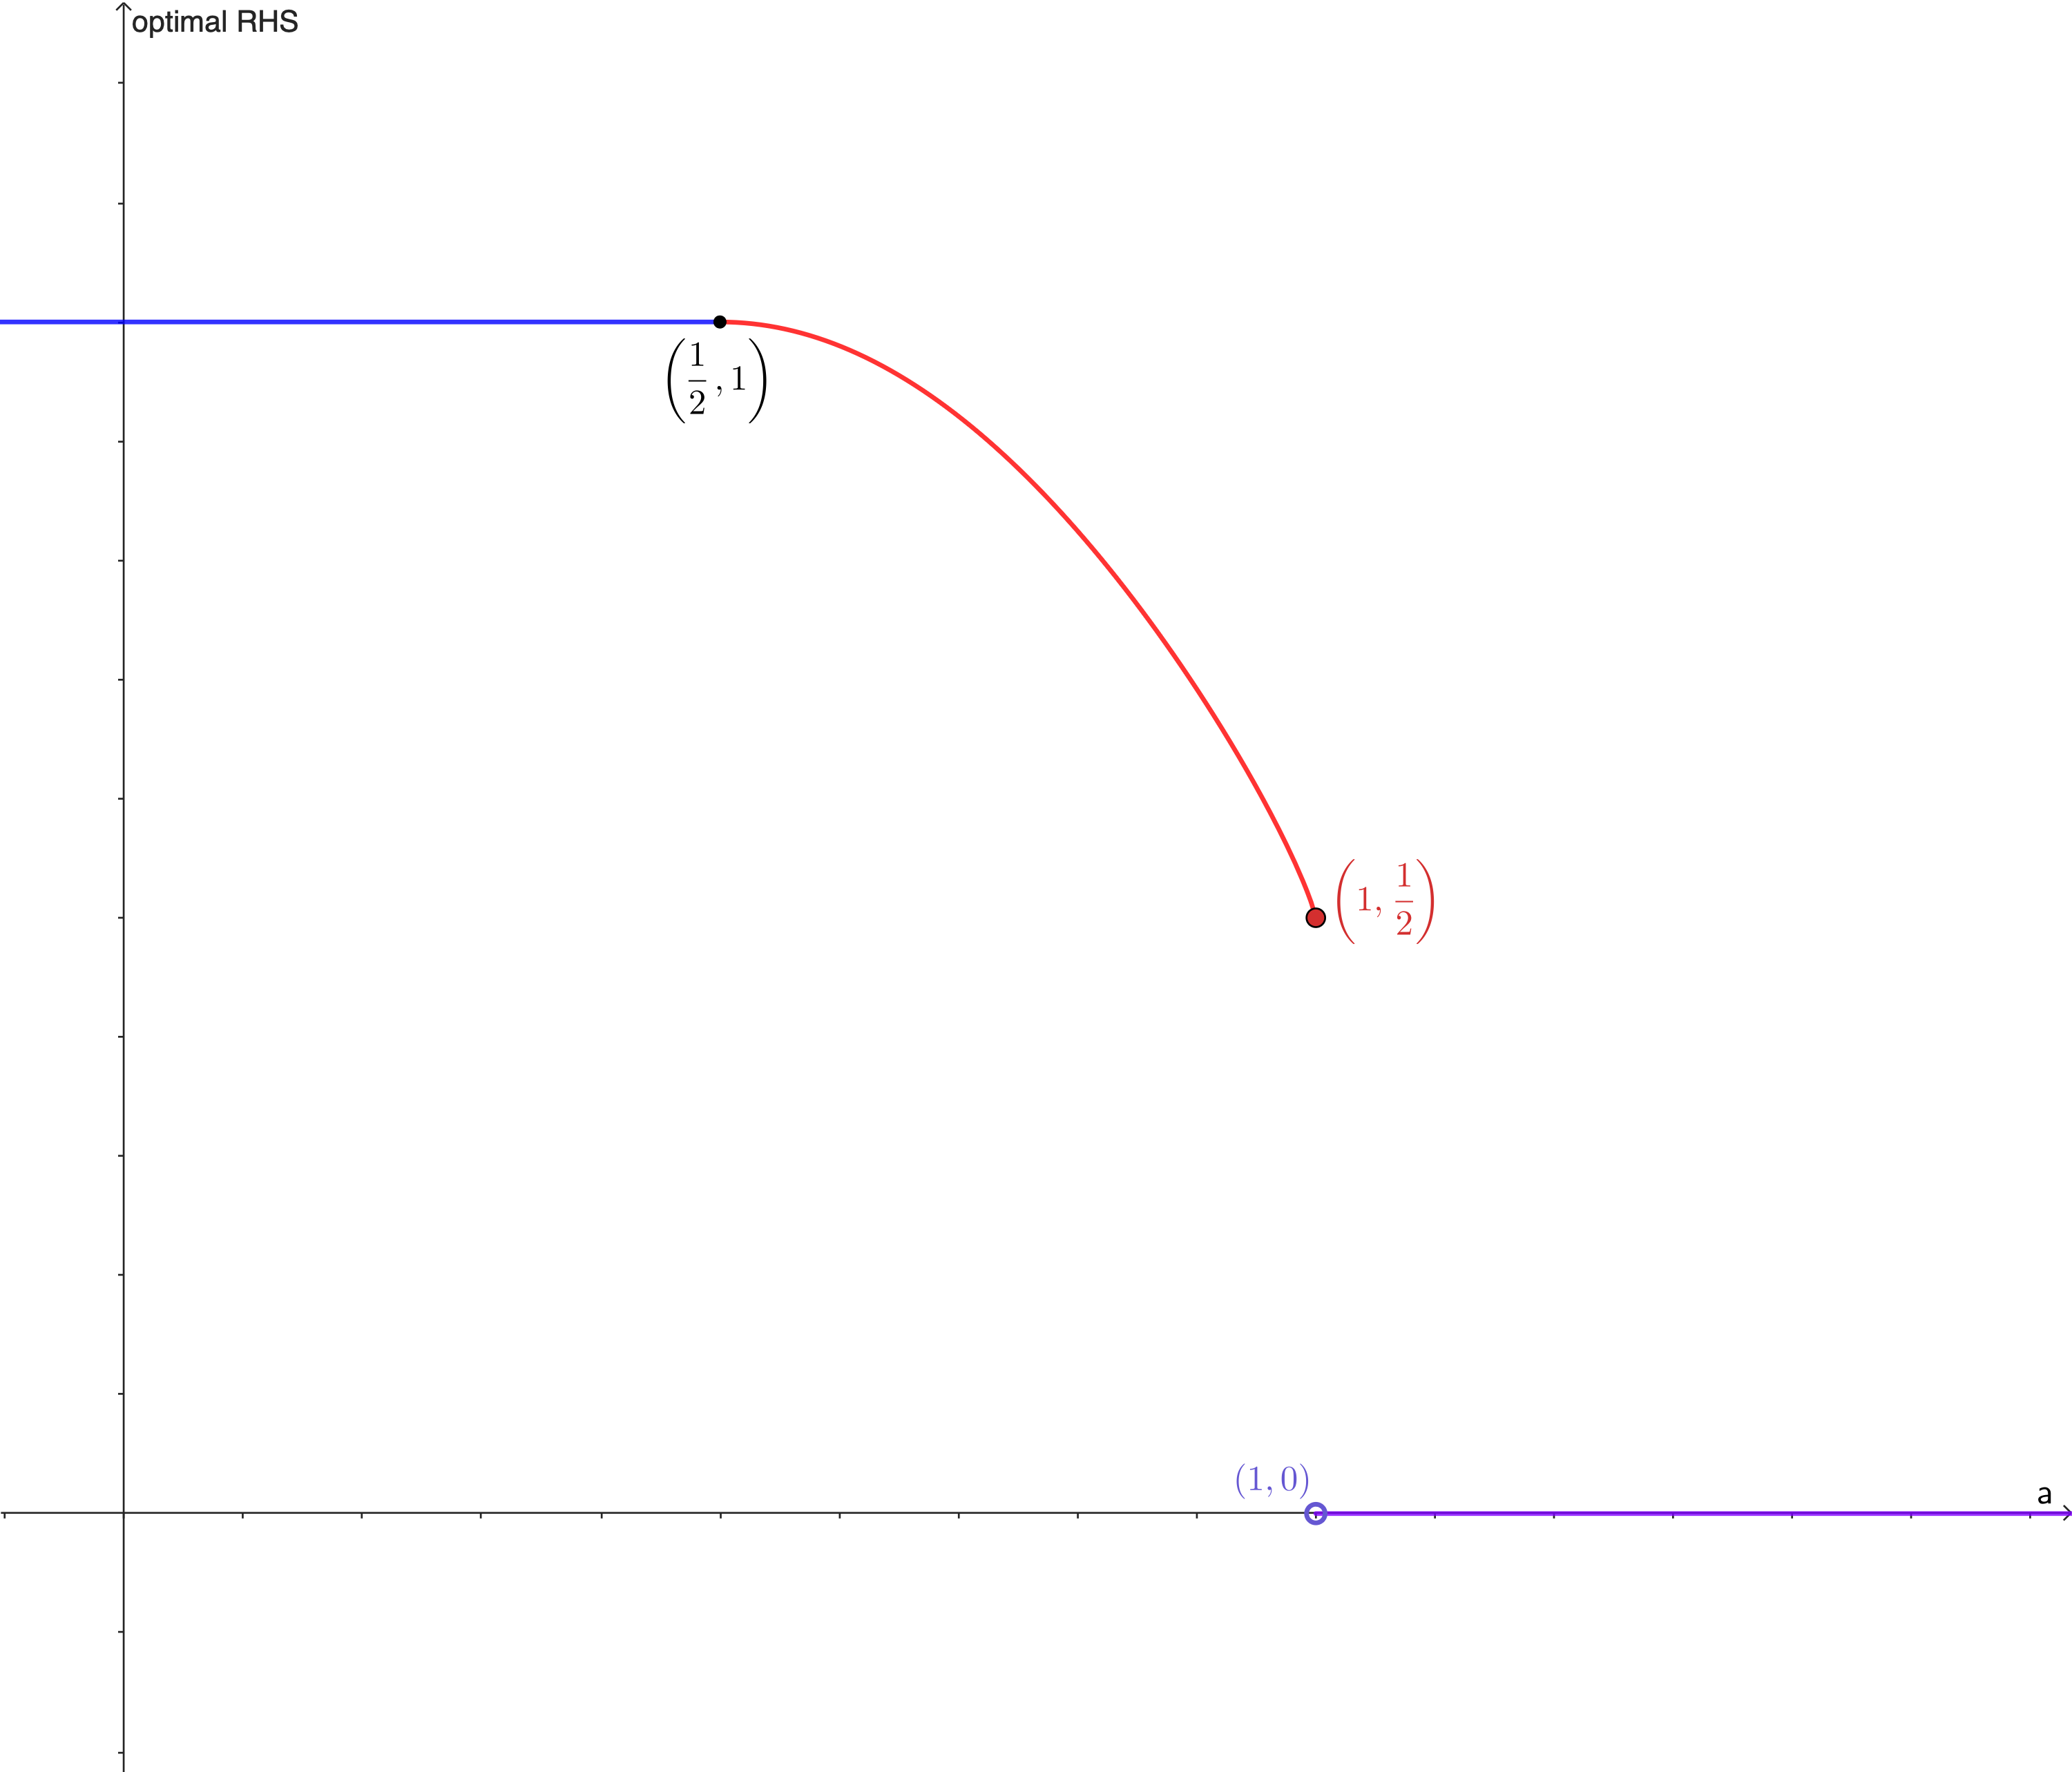
\includegraphics[width=0.45\linewidth]{bernouli}~~~~~~~h~~~
%\end{wrapfigure}
%\begin{wrapfigure}{c}{0.7\linewidth}
%\centering
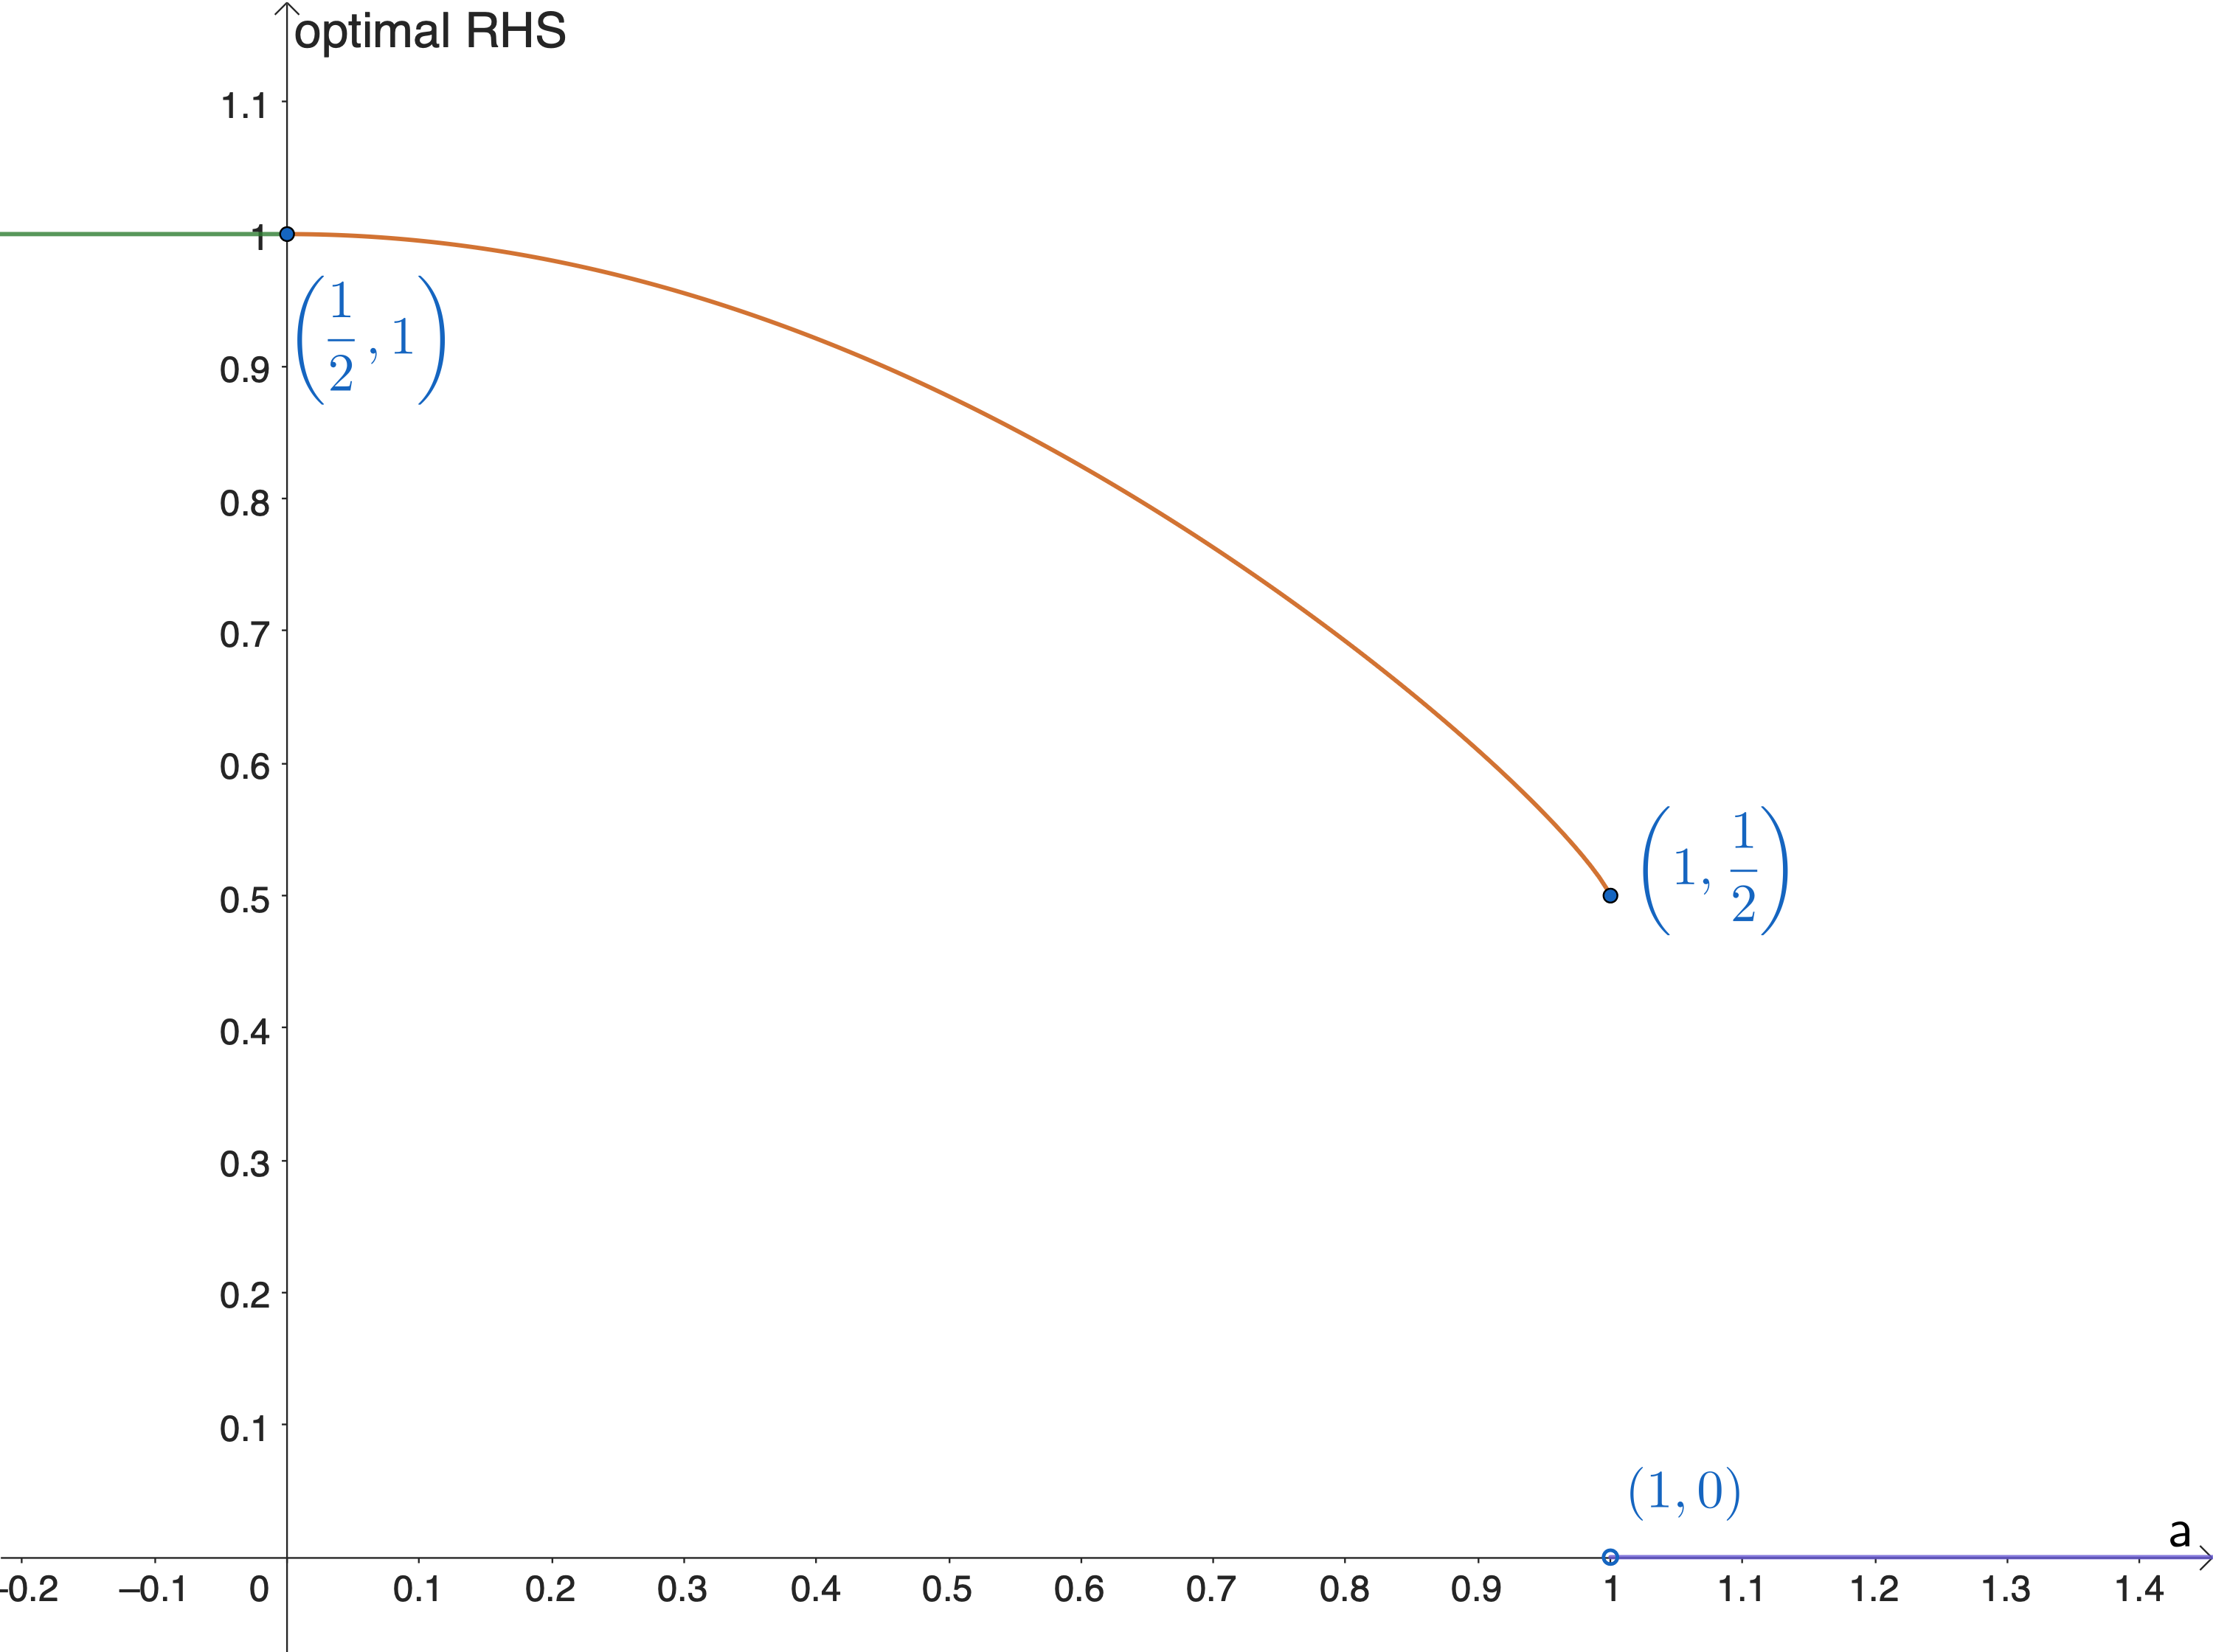
\includegraphics[width=0.45\linewidth]{rademacher}
\end{figure}

\subsection{Sub-Gaussian random variables}

Now let's apply it to our favorite distribution -- the Gaussian. Recall that the Gaussian distribution $Z$ with mean $\mu$ and variance $\sigma^{2}$ has the density $\ds f(x) = \frac{1}{\sigma\sqrt{2\pi}} \exp\left(\frac{-(x-\mu)^{2}}{2\sigma^{2}}\right).$ The moment generating function of this Gaussian is $M(t) = \exp\left(\mu t + \frac{\sigma^{2}t^{2}}{2}\right)$ and exists $\fa t\in\R$. Substituting this into our `moment-based Markov inequality' gives $\ds\P{Z\ge \mu+a} \le \inf_{t\ge 0} \exp\left(\frac{\sigma^{2}t^{2}}{2}-at\right) = \exp\left(-\frac{a^{2}}{2\sigma^{2}}\right)$. This means $\P{\abs{Z-\mu} \ge a} \le 2 \exp\left(-\frac{a^{2}}{2\sigma^{2}}\right)$ for any $a\ge 0$. 

This calculation let's us study the deviation of a large class of random variables, if this class is defined properly. If we revisit the calculation done for the Gaussian, we see that the only necessary property of any random variable $X$ that can get the same bound is the existence of some $\sigma^{2}$ such that we can get a similar function as an upper bound on the mgf of $X$. More precisely, we demand that there exist a real number $\sigma > 0$ such that $\E{\exp(t(X-\E X))} \le \exp\left(\frac{t^{2}\sigma^{2}}{2}\right)\fa t\in\R$. Alternately, instead of using the proof and calculation details, one might suggest to study those class of random variables whose deviations are bounded by those of the Gaussian. They turn out to be the same.

\begin{defn}
A random variable $X$ with mean $\mu$ is said to be \textit{sub-Gaussian} if there is a constant $c>0$ and a Gaussian $Z\sim \cN(0,\tau^{2})$ such that $\P{\abs {X-\mu}\ge a} \le c~\P{\abs Z \ge a}\fa a\ge 0$.

Alternately, a random variable $X$ with mean $\mu$ is said to be \textit{sub-Gaussian} if there exists $\sigma>0$ such that $\E{\exp(t(X-\E X))} \le \exp\left(\frac{t^{2}\sigma^{2}}{2}\right)\fa t\in\R$. This $\sigma^{2}$ is said to be the sub-Gaussian parameter and acts as a proxy for variance.
\end{defn}

This is quite a nice class because sub-Gaussianity is preserved under linear combinations. In particular, if $X_{1},X_{2}$ are independent sub-Gaussians with parameters $\sigma_{1}^{2},\sigma_{2}^{2}$ respectively then $X_{1}+X_{2}$ is also a sub-Gaussian with parameter $\sigma_{1}^{2}+\sigma_{2}^{2}$. In other words, the variance proxies add up just like the Gaussian. Using this property we immediately get


\begin{thm}[Hoeffding]
If $\set{X_{i}}_{i=1}^{m}$ are independent sub-Gaussians with means $\set{\mu_{i}}_{i=1}^{m}$ and variance proxies $\set{\sigma^{2}}_{i=1}^{m}$ respectively. Then 
$\ds\P{\sum_{i=1}^{m}(X_{i}-\mu_{i}) \ge t} \le \exp\set{-\frac{t^{2}}{2\sum_{i}\sigma_{i}^{2}}}$ for all $t\ge 0$.
\end{thm}

\begin{center}
\begin{tabular}{@{}l r}
\begin{minipage}[b]{0.5\textwidth}
At our current discussion stage, sub-Gaussians seem quite useless. But, a lot of the `good' random variables we see are actually sub-Gaussian. In fact if $X$ is a bounded random variable taking values in $[a,b]$ then $X$ is sub-Gaussian with parameter $\left(\frac{b-a}{2}\right)^{2}$. Here's a comparison of the bounds obtained with {\color{blue}fine analysis as in \Cref{rade}}  vs {\color{red}what the Hoeffding bound gives us}. Notice the smoothness difference.\end{minipage}&
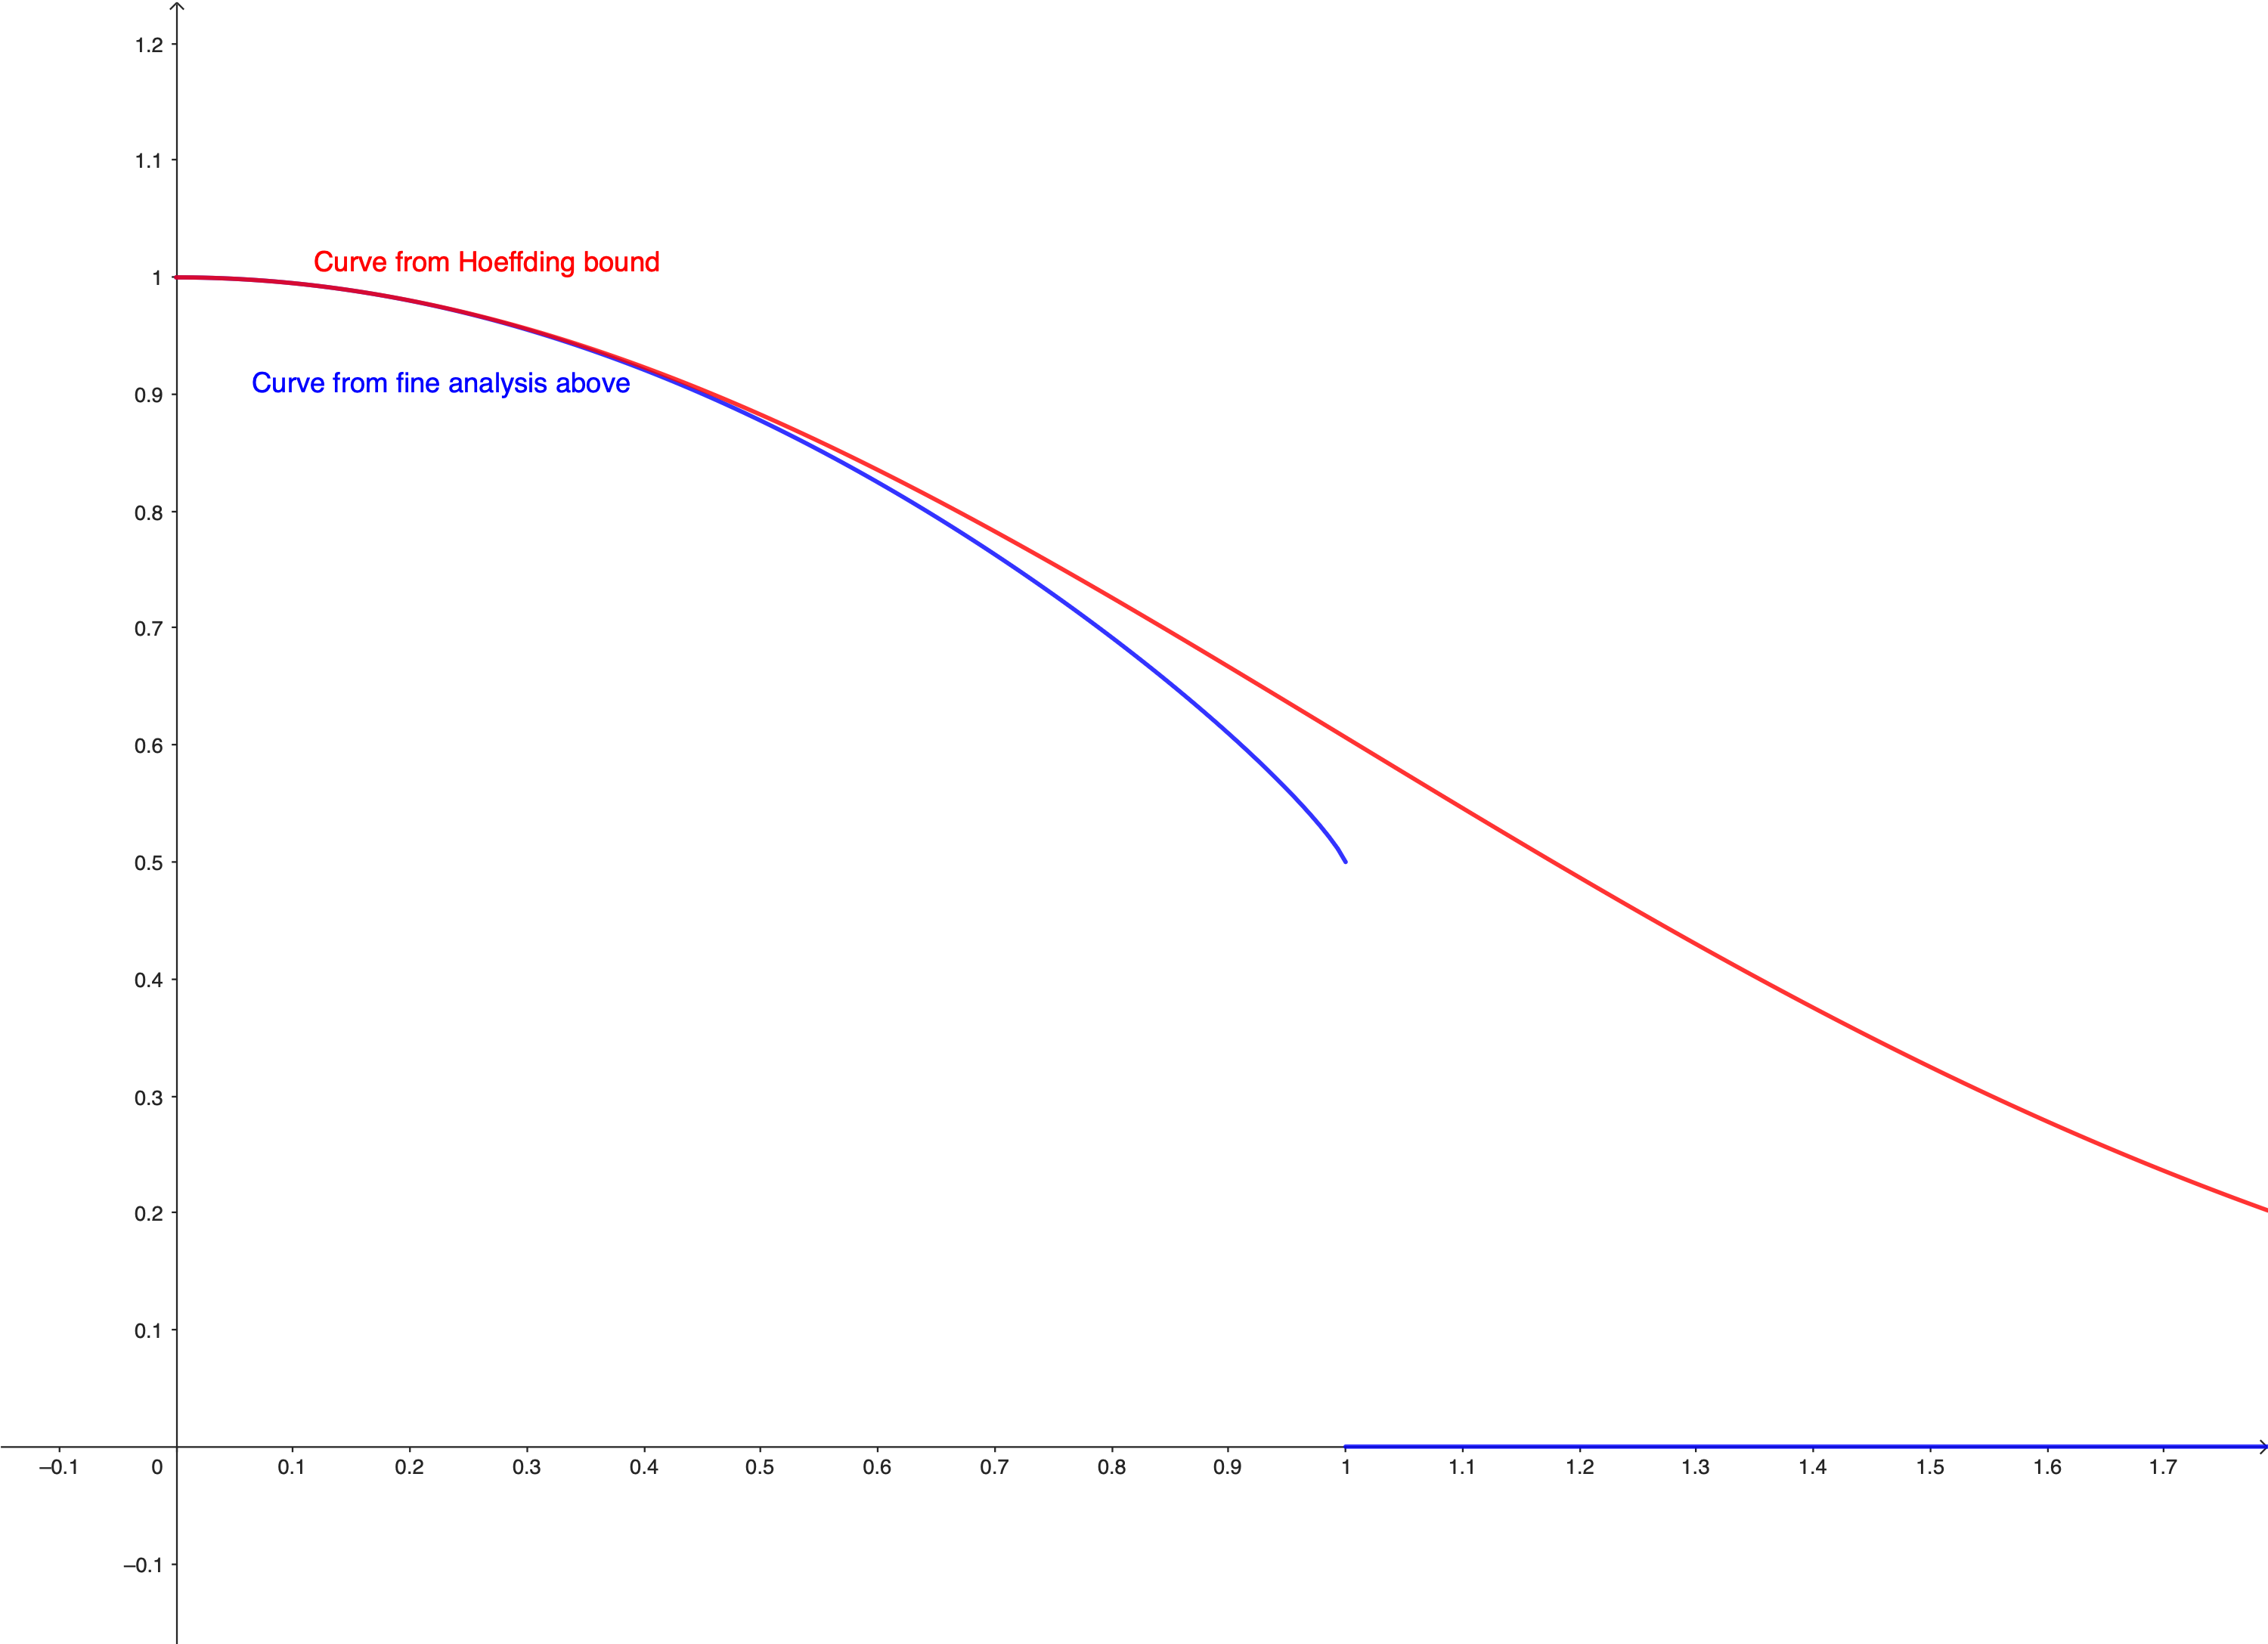
\includegraphics[width=3in]{compare} 
\end{tabular}
\end{center}

\begin{cor}
Let $X_{1},\cdots,X_{n}$ be independent bounded random variables such that $X_{i}\in[a_{i},b_{i}]$ (almost surely) and sample mean $\overline X$. Then $\ds\P{\overline X - \E{\overline X} \ge t} \le \exp\set{-\frac{2n^{2}t^{2}}{\sum_{i}(b_{i}-a_{i})^{2}}}$ for all $t\ge 0$.
\end{cor}



\section{Supervised Learning}
\paragraph{The setup.} In supervised learning, we are to design a \textit{learner} that learns the `labels' of certain `objects' or `data' and then we can use it to \textit{predict} unlabelled objects. An example could be a coin-sorting machine that understands (with human help) the sizes of various coins (data) and what size associates with what denomination (labels), and then when this model is released as a commercial product, the machine can speed up the process of sorting coins into different labelled stacks. 
\\
Formally, the data or inputs belong to some space $\cX$, and the labels are in some space $\cY$. For the above example, $\cX$ is the set of all coins and $\cY$ contains the string of labels of these coins like `dime', `nickel', `penny' and so on. We are interested in a certain joint probability distribution $\mathbb P$ over $\cX\times \cY$. A \textit{training set} is a finite (multi-)set of elements of $\cX\times \cY$ chosen independently and identically according to the distribution $\mathbb P$. We always denote this training set as $\set{z_{i}=(x_{i},y_{i})}_{i=1}^{n}$. Our goal is to design a \textit{model} $h:\cX\to\cY$, based on this training data, which has certain properties according to our needs. Such an $h$ is oftentimes also referred to as a \textit{hypothesis} or a \textit{predictor}. Note that a model can be \textbf{any} function $\cX\to\cY$.

\paragraph{Loss function.} How do we quantify the predictors which satisfy our needs. More precisely, when is a model better than another? For this, we have something called a \textit{loss function} $\l:{\color{red}\cY}\times {\color{blue}\cY} \to \R$ which is to be thought of as penalizing a {\color{red}predicted label} against the {\color{blue}actual label}. For example, the loss suffered by a model $h$ on a data point $x$ with label $y$ is $\l({\color{red}h(x)},{\color{blue}y})$ because $h(x)$ is the predicted label whereas $y$ is the actual label. Such a loss function is assumed to be non-negative. A `best' model is one which suffers the least expected loss. The expected loss of a model $h$ is $\ds L(h) \sett \underset{(x,y)\sim\mathbb P}{\mathbb E} \left[\l(h(x),y)\right]$, also called the \textit{population risk}. We want to find $\inf_{h} L(h)$.

\paragraph{Hypothesis class.} One question one might wonder is that what is the $\arg\min$ being taken over. In practice, we do not have a way of optimizing over arbitrary functions. We instead want to focus on a more specific subclass of functions which either make more sense in the context we are working on or are easier to work with. Such a constrained set of functions $\cH \subseteq \cY^{\cX}$ is called a \textit{hypothesis class}. Now we can clearly state a goal that we want to find $\ds\inf_{h\in\cH} \underset{(x,y)\sim\mathbb P}{\mathbb E} \left[\l(h(x),y)\right]$ (and find the minimizer if feasible or approximate it). This completes the formal setup of a supervised learning problem. This is impossible in general because we will not have access to $\mathbb P$ on the entire $\cX\times \cY$ but only to a finite sample. So we aim to design some $h\in \cH$ with minimum possible \textit{empirical loss}. In practice, we need to make assumptions and lots of restrictions on $\cH,\mathbb P, \l$ to get `good' results (whatever that means).

\paragraph{Examples.}
\begin{ex}[Binary classification]
In this case we want to classify objects in $\cX$ into two categories, so the label space is $\cY=\set{\square, \times}$. The usual penalization is given by the function $\l(\square, \times) = \l(\times,\square) = 1, \l(\square,\square)=\l(\times,\times)=0$. There is the classical problem of support vector machines. We describe a very simple but related problem. If $\cX\subseteq \R^{n}$, take $\cH=\set{\sgn(\inner{\pmb a}{\cdot} - b)\st \pmb a\in\R^{n}, b\in \R}$ where $\sgn(x) = \begin{cases}
\square & \text{ if } x\ge 0\\
\times & \text{ otherwise}
\end{cases}$. 
\end{ex}

\begin{ex}[Regression]
In the regression problem, we would like to predict continuous outputs $\cY=\R$ from a continuous input space $\cX = \R^{n}$. A popular loss function used in this case is $\l(y',y) = (y'-y)^{2}$. Other possible loss functions are $\l(y',y)=\abs{y'-y}^{p}$ for any $p\ge 0$ but $p=2$ is used in practice due to smoothness, convexity and low integer power. The hypothesis class depends on what kind of functions one thinks are fit for the model, again a choice to be made. Let's just focus on $\cH_{d} = \R[x_{1},\cdots,x_{n}]_{d}$ as the real polynomials in $n$ variables of degree at most $d$. If $d=1$, we call it \textit{linear regression}. If $d=2$ we call it quadratic regression. And so on.
\end{ex}

\paragraph{Empirical risk minimization.} Let's recall that our goal was to minimize the population risk, namely, $\ds\inf_{h\in\cH}\underset{(x,y)\sim\mathbb P}{\mathbb E} \left[\l(h(x),y)\right]$. In practice we do not have access to the entire
population; we only have a training set of $n$ data points, drawn independently from the same distribution as the entire population. To achieve our main goal, we can instead focus on the \textit{empirical risk} or \textit{sample risk} $\hat L(h) = \frac1n\sum\limits_{i=1}^{n}\l(h(x_{i}),y_{i})$. \textit{Empirical risk minimization}, or ERM in short, refers to finding $\ds\hat h \in \arg\min_{h\in\cH} \hat L(h)$. It is an unbiased estimator of the population risk. In other words, $\underset{z_{i}\stackrel{\text{iid}}{\sim} \mathbb P}{\mathbb E} \left[\hat L(h)\right] = L(h)$. The hope with ERM is that minimizing the empirical error will lead to small population error. So we are interested in the excess risk $\ds L\left(\hat h\right) - \inf_{h\in \cH}L(h)$. In other words, we are \textit{generalizing} the empirical risk minimizer to the population risk minimizer. One way to make this rigorous is by showing that the ERM minimizer’s excess risk is bounded. If $n$ is quite large, it makes sense to hope this intuitively due to the law of large numbers. 


\subsection{Non-asymptotic analysis} 

We do want non-asymptotic results when we have limited number of data points (that is, $n$ is relatively small). The LLN roughly states that the empirical average of a large number iid data behave as expected. In order to do the same for smaller-ish $n$, we study the concentration around the mean and hence we want to use concentration inequalities. Fortunately a lot of the distributions we deal with are, in real life, sub-Gaussian (or Lipschitz mappings of sub-Gaussians). But what we lose is that we can no longer make statements which are guaranteed to be true, but only bounds which hold `with high probability'. There is no clear definition of this term in literature but often used to refer to probabilities which are $\ge 1-\frac{1}{\text{poly}(n)}$.

Let me take a small detour and introduce a trick I learnt in my CS courses. Let $X_{j,1},\cdots, X_{j,n}\in [0,1]$ be independent for $k\in [K]$. Think of $j$ as the index of the person performing a repeated task. Denote their sample means by $Y_{j}\sett \frac{1}{n}\sum_{i}X_{ji}$ and $\mu_{j}\sett \E{Y_{j}}$. Then $\P{\underbrace{\abs{Y_{j}-\mu_{j}} \ge t}_{E_{j}\sett}} \le 2\exp\set{-2nt^{2}}\fa t\ge 0, j\in[K]$ by Hoeffding. If I want to find out the chance that even one of these random variables has large deviation from mean, I would consider the event $E \sett \bigcup\limits_{j\in[K]}\set{\abs{Y_{j}-\mu_{j}}\ge t} = \bigcup_{j}E_{j}$. Let's find the probability of this `bad' event. $\P{E} \le \sum_{j}\P{E_{j}} \le 2\sum_{j} \exp(-2nt^{2}) = 2K\exp(-2nt^{2})$. $\ds t = \sqrt{\frac{\ln(2K/\delta)}{2n}}$ gives $\P{\exists j\in[K] \text{ s.t. } \abs{Y_{j}-\mu_{j}} \ge \sqrt{\frac{\ln(2K/\delta)}{2n}}} \le \delta$. Taking complements, $$\P{\abs{Y_{j}-\mu_{j}} < \sqrt{\frac{\ln(2K/\delta)}{2n}}\fa j\in[K]} \ge 1-\delta.$$ In other words, we can make statements of the form ``with high probability, each person remains close to their expected behavior on average.'' Alternately taking $\ds n = \frac{\ln(2K/\delta)}{2\epsilon^{2}},$ $t=\epsilon$ gives $\P{\abs{Y_{j}-\mu_{j}} < \epsilon \fa j\in[K]} \ge 1-\delta.$ In other words, if every person performs $\ds \frac{\ln(2K/\delta)}{2\epsilon^{2}}$ experiments, each of their average behavior is expected to be within $\epsilon$ distance of the expected behavior with probability $1-\delta$.

Let's now consider this in the context of learning theory where the people are replaced with models $h\in \cH$. Recall that our main goal was to reach that the minimizer of ERM approximately minimizes the actual loss, that is, the excess risk $\ds L\left(\hat h\right) - \min_{h\in \cH}L(h)$ is quite small. If we can say with high certainty that every predictor is penalized almost as much on the population as the empirical data, we can conclude with high probability that the ERM minimizer also approximately minimizes the population risk. This is seen as follows.

\subsubsection{Finite hypothesis class}

\begin{prop}\label{prop:gen}
If every model $h\in \cH$ has almost the same penalization on the population as the sample, that is $\abs{L(h)-\hat L(h)} \le \frac{\epsilon}{2}$, then an ERM $\hat h \in \arg\min\limits_{h\in\cH} \hat L(h)$ minimizes $L$ upto $\epsilon$ accuracy.
\end{prop}
\begin{proof}
Denote $h^{*}\sett \arg\min_{h\in\cH}L(h)$. We want an upper bound on $L\left(\hat h\right) - L\left(h^{*}\right)$. Let's write it a little differently. $L\left(\hat h\right) - L\left(h^{*}\right) = {\color{blue}L\left(\hat h\right) - \hat L\left(\hat h\right)} + {\color{orange}\hat L\left(\hat h\right) - \hat L(h^{*})} + {\color{magenta}\hat L(h^{*}) - L(h^{*})}$. Note ${\color{orange}\hat L\left(\hat h\right) - \hat L(h^{*})} \le 0$. So $L\left(\hat h\right) - L\left(h^{*}\right) \le \abs{{\color{blue}L\left(\hat h\right) - \hat L\left(\hat h\right)}} + \abs{{\color{magenta}\hat L(h^{*}) - L(h^{*})}}$. Using the hypothesis gives $L\left(\hat h\right) - L\left(h^{*}\right) \le 2\sup\limits_{h\in\cH} \abs{L(h)-\hat L(h)} \le \epsilon$.
\end{proof}

In simpler terms, a uniform upper bound on $\abs{L-\hat L}$ implies generalization of the ERM to the population risk minimizer. Note that if we did not know a uniform upper bound on $\abs{L-\hat L}$, we could have still bounded $\abs{{\color{magenta}\hat L(h^{*}) - L(h^{*})}}$ via Hoeffding bound (with high probability). However, $\abs{{\color{blue}L\left(\hat h\right) - \hat L\left(\hat h\right)}}$ is data dependent (due to the data dependency of $\hat h$). It is quite possible that this term is quite big. In fact it's often practically encountered if $\cH$ is not chosen carefully -- even with small training error, there can be large testing error. 

\begin{cor}
For a finite hypothesis class $\cH$, a loss function $\l\in[0,1]$ with $n$ training data points and $\delta\in(0,0.5)$, we have $\ds\P{\abs{L(h)-\hat L(h)} < \sqrt{\frac{1}{2n}\ln \left(\frac{2\abs{{\cH}}}{\delta}\right)}\fa h\in\cH} \ge 1-\delta.$ \\
Consequently, $\P{\abs{L\left(\hat h\right)- L(h^{*})} < \sqrt{\frac{2}{n}\ln \left(\frac{2\abs{{\cH}}}{\delta}\right)}} \ge 1-\delta.$
\end{cor}
\begin{proof}
The first part is proven the same way as the trick discussed in the previous page with people being replaced by models $h$, $K = \abs{\cH}$ and the random variables being the evaluation of $\l$ on the training data. The second part is immediate by \Cref{prop:gen}.
\end{proof}

\begin{cor}\label{cor:n}
For a finite hypothesis class $\cH$, a loss function $\l\in[0,1]$, $\delta\in(0,0.5)$, and (additive) error tolerance $\epsilon>0$, it is enough to have $\ds n=\cO\left(\frac{2}{\epsilon^{2}}\ln\left(\frac{2\abs {\cH}}{\delta}\right)\right)$ training data points to achieve $\epsilon$-generalization of ERM to population risk minimum with probability $1-\delta$. 
\end{cor}

\begin{cor}\label{cor:delta}
For a finite hypothesis class $\cH$, a loss function $\l\in[0,1]$, (additive) error tolerance $\epsilon>0$ and $n$ samples, $\abs{L(h)-\hat L(h)} < \epsilon\fa h\in \cH$ with probability $\ds\ge 1-2\abs{\cH}\exp(-2n\epsilon^{2})$.
\end{cor}

\subsubsection{Infinite hypothesis class}
The above analysis relied heavily on the size of $\cH$. This cannot be done when $\cH$ is infinite, which it usually is. Unless we assume some structure on $\cH$, it's quite difficult to do the analysis for infinite $\cH$. So we will assume that $\cH$ is bounded with some bounded parameters, usually taken to be vectors in $\R^{p}$. That is we will have $B>0$ such that $\cH=\set{h_{\theta} \st \theta\in\R^{p}, \norm{\theta}{2}\le B}$. $\Theta \sett \set{\theta\in\R^{p}, \norm{\theta}{2}\le B}$ is the parameter space for $\theta$'s. The technique to be used here is called \textit{brute-forced discretization}. Here's the main idea.

Let's abuse notation and write $L(\theta),\hat L(\theta)$ for $L(h_{\theta}),\hat L(h_{\theta})$ respectively. As before, we name the `bad' events $E_{\theta} \sett \set{L(\theta) - \hat L(\theta) \ge \epsilon}$. If we want to use the previous technique, we end up in the situation $\P{\bigcup\limits_{\theta\in\Theta}E_{\theta}} \le \sum\limits_{\theta\in\Theta}\P{E_{\theta}}$ where the sum is an infinite sum of finite quantities whose known upper bounds (via the Hoeffding bound) are all equal. However, if we know that `nearby' $\theta$'s give `nearly the same' losses, we can choose some prototype candidates $\theta_{1},\cdots,\theta_{N}\in \Theta$ so that every $\theta\in\Theta$ is `near' some $\theta_{i}$. This way, we have discretized $\Theta$. Now a standard union bound + Hoeffding trick on these prototype $\theta_{i}$'s will do the job because there's only finitely many of them and they approximate the global behavior of the loss for all $\theta\in\Theta$. Let's make these precise.

The `nearness' of the prototype $\theta_{i}$'s is made rigorous through what is called an $r-$net.
\begin{defn}[$r-$net]
Let $\epsilon>0$ and $S$ a subset of a metric space $(X,d)$. The closed ball of radius $r$ around $x\in X$ will be denoted by $D_{r}(x) = \set{y\in X\st d(x,y)\le r}$. An \textit{$r-$net of $S$} is a subset $T_{r}\subseteq S$ such that for each $x\in S$ there is some $y\in T_{r}$ satisfying $d(x,y)\le r$. In other words, $S \subseteq \bigcup\limits_{x\in T_{r}}D_{r}(x)$.
\end{defn}

Now we need to find an $r-$net of $\Theta$ which is not only finite, but also not too large in size, otherwise the union bound + Hoeffding trick would not work. We are in luck because there is an $r-$net of $\Theta = \set{\theta\in\R^{p} \st \norm \theta2\le B}$ of size $\ds\le\left(\frac{3B}{r}\right)^{p}$. We'll prove this later.

Now let's make the idea of ``nearby $\theta$'s give nearly the same loss'' precise, which will be an added assumption on the loss function. Recall that the loss of $h_{\theta}$ on $(x,y)$ is $\l(h_{\theta}(x),y)$. This value actually depends on three things, namely $\theta,x,y$. We would like that for the same data point $(x,y)$, changing the parameters of the model only a little bit does not change the loss by much. That is, for any $(x,y)$, if we change the parameters only slightly, the change in the penalty is controlled. This is captured by something called Lipschitz-ness. A Lipschitz function is continuous, but not necessarily differentiable. All we can say is that Lipschitz functions are almost everywhere differentiable.
\begin{defn}[$\kappa-$Lipschitz]
A real. valued function $f:X\to \R$ on a metric space $(X,d)$ is said to be \textit{$\kappa-$Lipschitz} if $\abs{f(x) - f(y)} \le \kappa d(x,y)$ for every $x,y\in X$.
\end{defn}

Let's now try to imitate the calculations as before, incorporating the Lipschitzness of the loss function and see how things turn out. Say, the loss $\l$ takes values in $[0,1]$ and is $\kappa-$Lipschitz in $\theta$ with the usual $\l_{2}$ norm on $\R^{p}$, that is, $\abs{\l(h_{\theta}(x),y)-\l(h_{\theta'}(x),y)} \le \kappa \norm{\theta-\theta'}{2}$. Consequently, $L,\hat L$ are also $\kappa-$Lipschitz. Since we already have an $r-$net $T$ for $\Theta\subseteq \R^{p}$ of size $\ds N\le \left(\frac{3B}{r}\right)^{p}$, let's just focus on the loss values on these points, which approximate the other points in its neighborhood. Say $T = \set{\theta_{1},\cdots,\theta_{N}}$. So we are interested in the good event $E = \set{\abs{L(\theta_{i})-\hat L(\theta_{i})} < \frac{\epsilon}2 \fa i\in[N]}$. We put $\epsilon/2$ instead of $\epsilon$ in order to account for the errors caused by approximation of points in $\Theta$ outside $T$. By \Cref{cor:delta}, $\P{E} \ge 1-2N\exp(-n\epsilon^{2}/2)$. We have thus obtained a uniform upper bound for $\abs{L-\hat L}$ on $T$ with high probability. Let's extend this to $\Theta$. Indeed for any $\theta\in \Theta$, there is some $x\in T$ such that $\norm{\theta-x}{2}\le r$. Recall that $L,\hat L$ are $\kappa-$Lipschitz. Thus conditioned on $E$, $\abs{L(\theta)-\hat L(\theta)} \le \abs{L(\theta)-L(x)} + \abs{L(x)-\hat L(x)} + \abs{\hat L(x)-\hat L(\theta)} \le 2\kappa r + \frac{\epsilon}2$. 

\begin{thm}
Suppose we are given an hypothesis class $\cH$ parameterized by $\Theta=\set{\theta \in\R^{p}\st \norm \theta2\le B}$, a loss function $\l$ taking values in $[0,1]$ and $\kappa-$Lipschitz on model parameters $\theta$, $n$ training samples and an (additive) error tolerance $\epsilon>0$.\\ 
Then $\ds \P{\abs{L(\theta)-\hat L(\theta)} < \epsilon\fa \theta\in \Theta} \ge 1 - 2\left(\frac{18B\kappa}{\epsilon}\right)^{p}\exp(-2n\epsilon^{2})$.
\end{thm}
\begin{proof}
Choose $\ds r = \frac{\epsilon}{5\kappa}$ in the above discussion.
\end{proof}

\begin{thm}
Suppose we are given an hypothesis class $\cH$ parameterized by $\Theta=\set{\theta \in\R^{p}\st \norm \theta2\le B}$, a loss function $\l$ taking values in $[0,1]$ and $\kappa-$Lipschitz on model parameters $\theta$ and $n$ training samples.\\ 
Then $\ds \P{\abs{L(\theta)-\hat L(\theta)} < \cO\left(\sqrt{\frac{p \max\set{1,\ln(\kappa Bn)}}{n}}\right)\fa \theta\in \Theta} \ge 1 - \cO(\exp(-\Omega(p)))$.
\end{thm}

\begin{cor}
Suppose we are given an hypothesis class $\cH$ parameterized by $\Theta=\set{\theta \in\R^{p}\st \norm \theta2\le B}$, a loss function $\l$ taking values in $[0,1]$ and $\kappa-$Lipschitz on model parameters $\theta$, $\delta\in(0,0.5)$ and an (additive) error tolerance $\epsilon>0$. Then it is enough to have a training sample set of size $\ds n = \cO\left(\frac{\ln(2/\delta) + p \max\set{1,\ln(18B\kappa/\epsilon)}}{2\epsilon^{2}}\right)$ to guarantee $\abs{L(\theta)-\hat L(\theta)} < \epsilon\fa \theta\in \Theta$ with probability at least $1 - \delta$.
\end{cor}

\newpage 
We end with an upper bound for an $r-$net of $\Theta$ for $r\le B$. In what follows, $B,B^{o}$ will respectively denote closed and open balls. 

Consider the following algorithm for any given $r>0$ to find a set $T_{r}\subseteq \Theta$. 
\begin{algorithmic}[1]
\Require $r>0,$ dimension $p$
\Ensure a number $N$ and points $\pmb v_{1},\cdots,\pmb v_{N}\in \Theta$ such that every point in $\Theta$ is $r-$close to some $\pmb v_{i}$.
\Begin
\State $N\gets 1$
\State $\pmb v_{1} \gets (1,0,\cdots,0)\in\Theta$
\State $T \gets B_{r}^{o}(\pmb v_{1})\cap \Theta$ \Comment{points in $\Theta$ which are at distance $<\epsilon$ from $\pmb v_{1}$}
\While {$N\geq 1$} 
    \State $\pmb v_{N} \gets $any point in $\Theta\smallsetminus T$
    \State $T \gets T\cup (B_{r}(\pmb v_{2})\cap \Theta)$
    \If{$S=\Theta$} \Comment{check if $\Theta$ has been covered}
    	\State \textbf{break}
	\Else
		\State $N \gets N+1$
	\EndIf
\EndWhile 
\State \Return $N,T_{r} = \set{\pmb v_{1},\cdots,\pmb v_{N}}$
\End
\end{algorithmic}

Now we prove that this algorithm actually gives $T_{r}$ and size $N$ as desired. 
If the above algorithm terminates with answer $N,T_{r}$, then $\Theta\subseteq \bigcup\limits_{i=1}^{N}B_{r}^{o}(\pmb v_{i}) \subseteq \bigcup\limits_{i=1}^{N}B_{r}(\pmb v_{i})$.

\begin{cl}
The above algorithm terminates.
\end{cl}
\begin{proof}
Suppose the algorithm goes on forever. So we get a sequence of points $\pmb v_{1}, \pmb v_{2},\cdots$ such that $\Theta \subseteq \bigcup\limits_{i\in\N}B_{r}^{o}(\pmb v_{i})$. Since $\Theta$ is compact there is a finite $N$ such that $\Theta\subseteq \bigcup\limits_{i=1}^{N}B_{r}^{o}(\pmb v_{i})$. This is a contradiction to our original assumption.
\end{proof}

Next we note that just by how our algorithm is designed, if $\pmb x,\pmb y\in T_{r}$ then $\norm{\pmb x-\pmb y}{2}\ge r$. This is because a new point (line $6$) is always chosen so that it is not in the $r-$ball around any of the previously chosen points, and distance is symmetric.

Further $T_{r}$ is maximal in the sense that if $T'\supsetneq T_{r}$ is a collection of points in $\Theta$, there will be two points in $T'$ which are at most $r-$close to each other. This is by our breaking criterion on line $8$. Simply put, $T_{r}$ covers $\Theta$ with $\epsilon-$balls.

\begin{cl}\label{disj}
If $\pmb x,\pmb y\in T_{r}$ are distinct, then $B_{\frac{r}{2}}^{o}(\pmb x)\cap B_{\frac{r}{2}}^{o}(\pmb y) \cap \Theta = \varnothing$.
\end{cl}
\begin{proof}
Suppose $\pmb p\in \Theta\cap B_{\frac{r}{2}}^{o}(\pmb x)\cap B_{\frac{r}{2}}^{o}(\pmb y)$ and say $\pmb y$ was picked after $\pmb x$ in the algorithm. Then $\norm{\pmb x-\pmb y}{2}\le \norm{\pmb x-\pmb p}{2} + \norm{\pmb p-\pmb y}{2} \le r$. Moreover equality here occurs only when $\norm{\pmb p-\pmb x}{2} = \norm{\pmb p-\pmb y}{2}=\frac{r}{2}$ which means $p\notin B_{\frac r2}^{o}(\pmb x)$ which is a contradiction. So it must happen that $\norm{\pmb x-\pmb y}2<r$ which contradicts the constructive step in line $6$ because this indicated that $\pmb y$ was picked in the $r-$ball around $\pmb x$.
\end{proof}

\begin{cl}\label{ball}
For any $t\ge 0$, if $\pmb x\in \bigcup\limits_{i\in [N]}B_{t}(\pmb v_{i})\subseteq \R^{n}$ then $\norm{\pmb x}{2}\le B+t$.
\end{cl}
\begin{proof}
Say $\pmb x\in B_{t}(\pmb v_{i})$ for some $i$. Then 
$\norm{\pmb x}2 \le \norm{\pmb v}2 + \norm{\pmb x-\pmb v}{2} \le B+t.$
\end{proof}

The last two claims show that $\ds X\sett\bigcup\limits_{i\in [N]}B_{r/2}(\pmb v_{i})$ is an almost disjoint union and is contained in the closed ball of radius $B+\frac r2$. The volume of a ball of radius $t$ in $\R^{p}$ is $c_{p}t^{p}$ where $c_{p}$ is a constant depending only on $p$. Thus $N(r/2)^{p} \le (B+r/2)^{p}$ whence $N\le \left(\frac{2B}{r}+1\right)^{p} \le \left(\frac{3B}{r}\right)^{p}$ whenever $r\le B$.









\nocite{*}
\printbibliography

















\end{document}

